\documentclass[10pt]{beamer}
\usepackage[utf8]{inputenc}
\usepackage[francais]{babel}
\usepackage[T1]{fontenc}
\usepackage[export]{adjustbox}
\newcommand\Fontvi{\fontsize{8}{7.2}\selectfont}

\usepackage{minted}
\usemintedstyle{colorful}
\usepackage{hyperref}
\hypersetup{
	colorlinks,
	citecolor=black,
	filecolor=black,
	linkcolor=black,
	urlcolor=blue
}

\usetheme{Frankfurt}
\usecolortheme{beaver}

\addtobeamertemplate{navigation symbols}{}{%
    \usebeamerfont{footline}%
    \usebeamercolor[fg]{footline}%
    \hspace{1em}%
    \insertframenumber/\inserttotalframenumber
}

\begin{document}
\logo{%
	\makebox[0.95\paperwidth]{%
		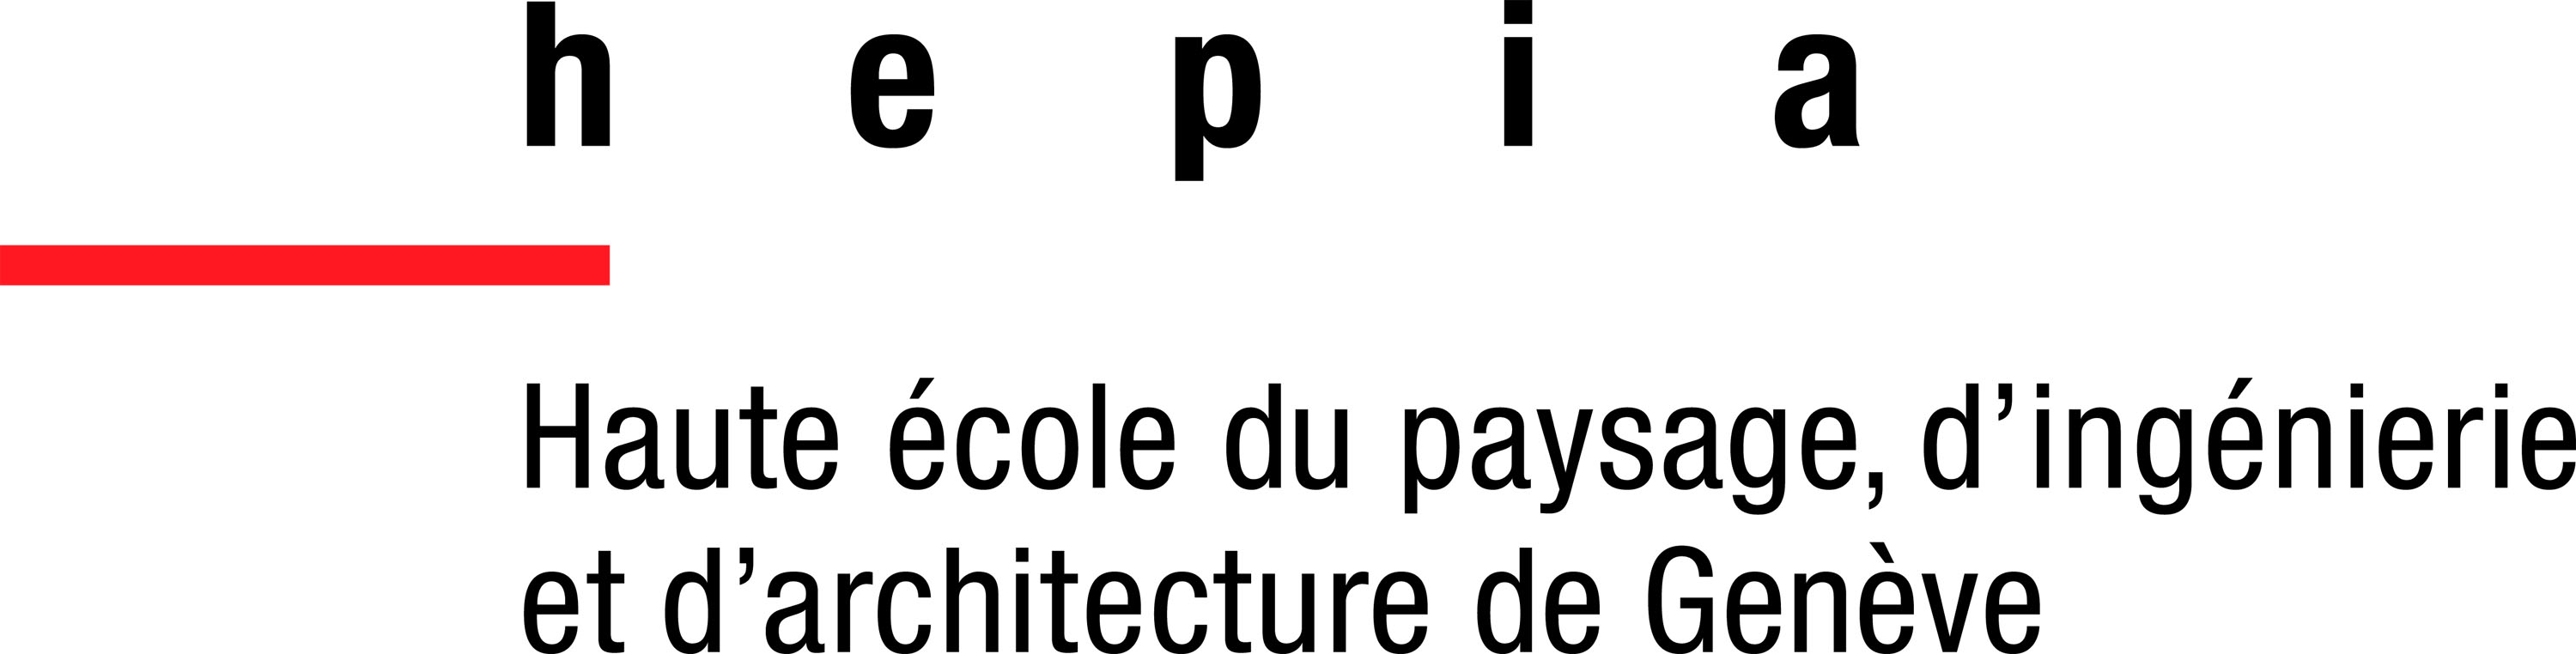
\includegraphics[width=2.5cm,keepaspectratio]{images/hepia.jpg}%
		\hfill%
		
\includegraphics[width=2.5cm,keepaspectratio]{images/hesso.jpg}%
	}%
}

\title{Festival Search Engine}
\author{Steven Liatti et Vincent Tournier}
\institute{Cours de systèmes distribués - Prof. Nabil Abdennadher - Hepia ITI 3\up{ème} année}
\date{13 décembre 2017}

\begin{frame}
\titlepage
\end{frame}

\begin{frame}
	\setcounter{tocdepth}{2}
    \frametitle{Plan}
    \begin{columns}[t]
        \begin{column}{.5\textwidth}
            \tableofcontents[sections={1-2}]
        \end{column}
        \begin{column}{.5\textwidth}
            \tableofcontents[sections={3-4}]
        \end{column}
    \end{columns}
\end{frame}



\section{Introduction}
\subsection{Buts du projet}
\begin{frame}
	\frametitle{\secname}
	\framesubtitle{\subsecname}
	Créer un moteur de recherche d'événements musicaux, permettant à l'utilisateur de :
	\begin{itemize}
		\item Afficher des événements sur une carte interactive
		\item Afficher des informations d'un événement en particulier
		\item Afficher des informations à propos des artistes
		\item Jouer (en arrière plan) un extrait d'un son d'un artiste de l'événement
	\end{itemize}
\end{frame}
\subsection{API utilisées}
\begin{frame}
	\frametitle{\secname}
	\framesubtitle{\subsecname}
	\begin{itemize}
		\item Spotify : recherche d'artistes et top tracks (route \mintinline{text}{events}, \mintinline{text}{infos} et \mintinline{text}{tracks})
		\item Eventful : liste des événements (lieux, dates et artistes) (route \mintinline{text}{events})
		\item Wikipédia : principale source d'informations sur un artiste (route \mintinline{text}{infos})
        \item MusicBrainz : informations complémentaires sur les artistes (route \mintinline{text}{infos})
		\item BandsInTown : informations complémentaires sur les artistes (route \mintinline{text}{events} et \mintinline{text}{infos})
		\item Google Maps : pour la carte interactive côté client
	\end{itemize}
\end{frame}

\section{Serveur}

\subsection{Route \mintinline{text}{events}}
\begin{frame}
	\frametitle{\secname}
	\framesubtitle{\subsecname}
	\begin{figure}
		\begin{center}
			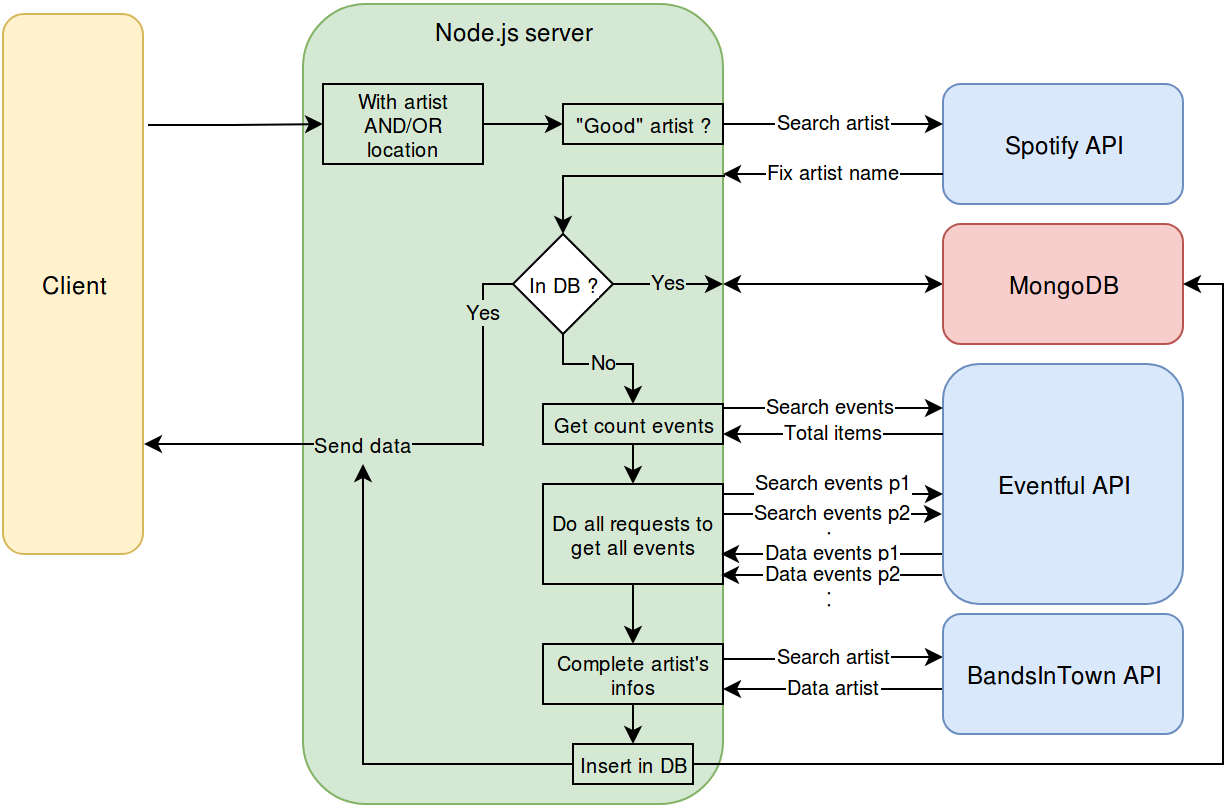
\includegraphics[width=0.8\textwidth]{images/events.png}
		\end{center}
		\caption{Route events}
	\end{figure}
\end{frame}

\subsection{Route \mintinline{text}{infos}}
\begin{frame}
	\frametitle{\secname}
	\framesubtitle{\subsecname}
	\begin{figure}
		\begin{center}
			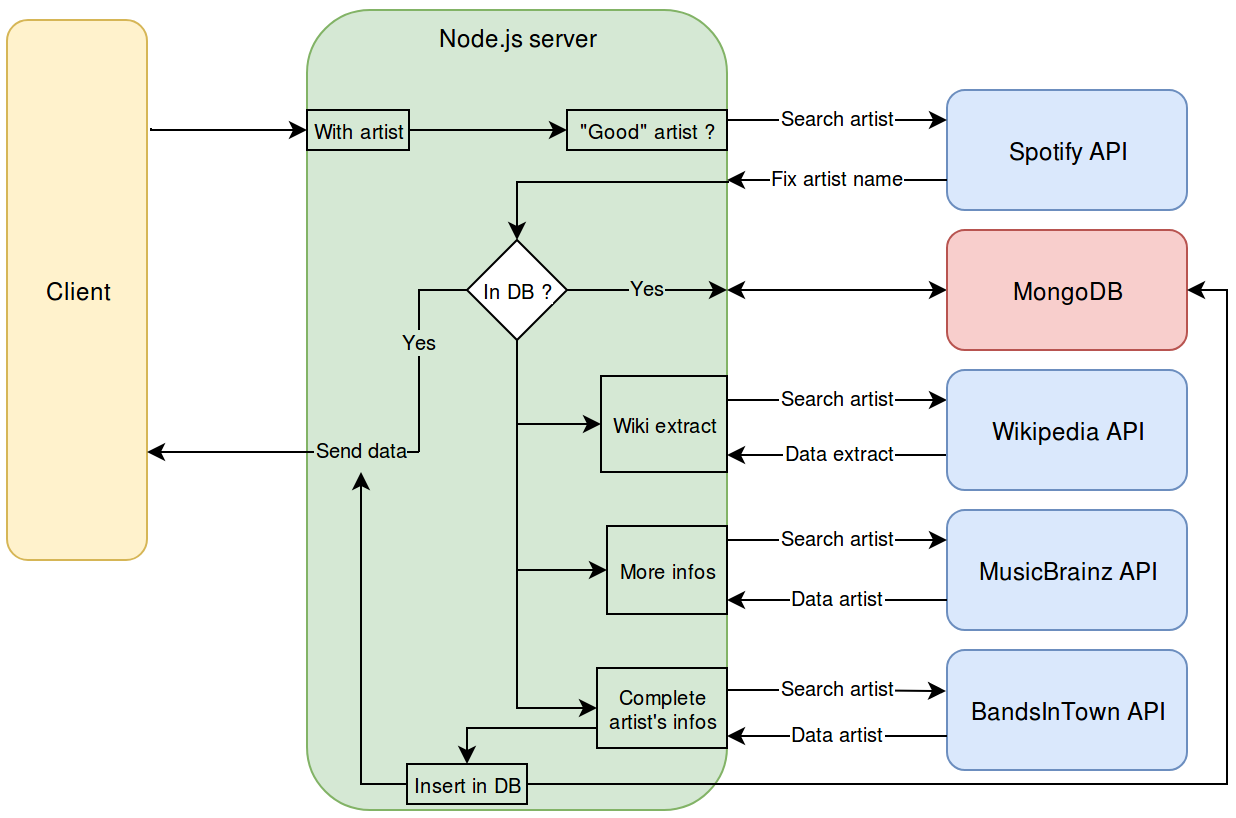
\includegraphics[width=0.8\textwidth]{images/infos.png}
		\end{center}
		\caption{Route infos}
	\end{figure}
\end{frame}

\subsection{Route \mintinline{text}{tracks}}
\begin{frame}
	\frametitle{\secname}
	\framesubtitle{\subsecname}
	\begin{figure}
		\begin{center}
			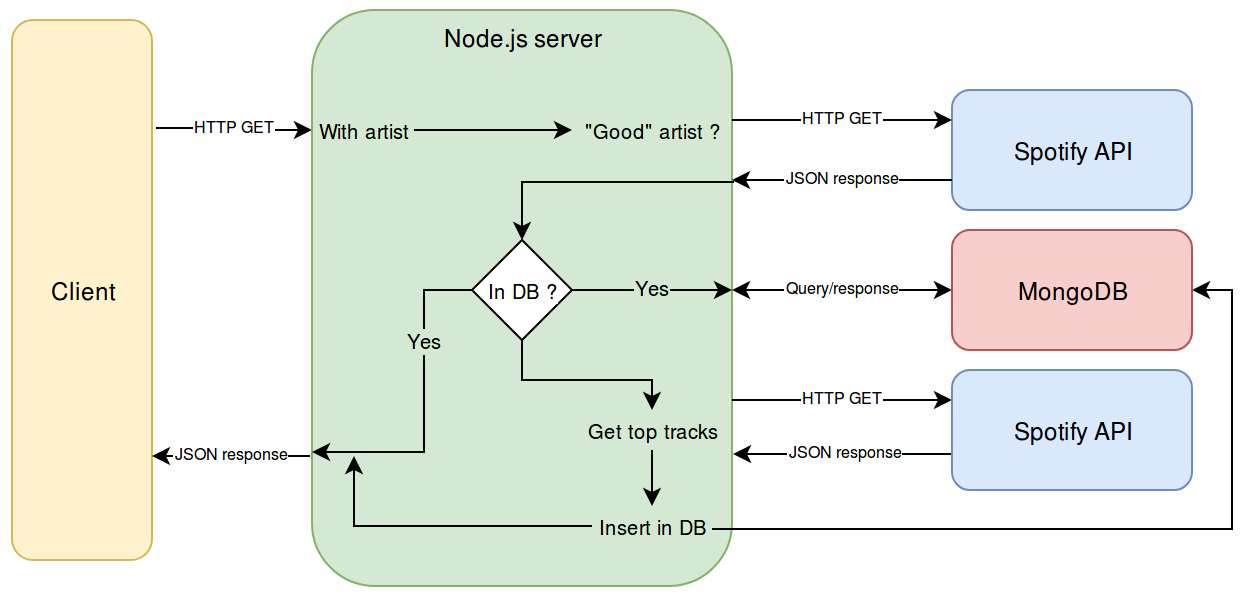
\includegraphics[width=0.8\textwidth]{images/tracks.png}
		\end{center}
		\caption{Route tracks}
	\end{figure}
\end{frame}

\subsection{MongoDB}
\begin{frame}
	\frametitle{\secname}
	\framesubtitle{\subsecname}
	Utilisation de MongoDB comme base de données :
	\begin{itemize}
		\item Simplicité/compatibilité avec Javascript et Node.js (JSON)
		\item Données "temporaires" avec la feature MongoDB Time To Live
		\item Découverte d'un SGBD alternatif (NoSQL)
	\end{itemize}
\end{frame}

\subsection{Divers}
\begin{frame}[fragile]
	\frametitle{\secname}
	\framesubtitle{\subsecname}
	Serveur Node.js avec structure basée sur les promesses (Promise) :
	\begin{minted}[linenos]{javascript}
// doSomething() and doSomethingElse() return a Promise
doSomething()
.then(result => { return doSomethingElse(result); })
.then(finalResult => { console.log("OK :" + finalResult); })
.catch(error => { console.log(error); });
	\end{minted}
	\bigbreak
	Utilisation d'AWS (avec scripts shell pour le déploiement) :
	\begin{itemize}
		\item Pour héberger le serveur Node.js, la base de données MongoDB,
		la documentation de l'API et le serveur Apache pour servir les fichiers client (HTML)
		\item Mettre en pratique le cours de Cloud
	\end{itemize}
\end{frame}

\section{Client}
\subsection{APIs & technologies}
\begin{frame}
	\frametitle{\secname}
	\begin{itemize}
		\item Javascript & JQuery
		\item Google Maps (Map, marker, infobubble, geocoder)
		\item Overlapping Marker Spiderfier
		\item Maps marker clusterer
	\end{itemize}
\end{frame}

\subsection{En gros}
\begin{frame}
	\frametitle{\secname}
	\begin{itemize}
		\item Un formulaire
		\item Pleins de <div>
		\item Deux arguments en URL
		\item Et du script
	\end{itemize}
\end{frame}

\section{Conclusion}
\begin{frame}
	\frametitle{\secname}
	Steven :
	\begin{itemize}
		\item Approfondissement de Node.js et découverte des Promise Javascript et de MongoDB
		\item Découverte de bonnes (Spotify, Wikipédia) et "moins bonnes" (MusicBrainz, Eventful) API
	\end{itemize}
	Vincent :
	\begin{itemize}
		\item
	\end{itemize}
	\Large\textbf{Beaucoup de plaisir à travailler sur ce projet}
\end{frame}

\end{document}
